\section{Randomness and Super-Sampling}
TODO: maybe this subsection is unimportant

It is important to note that if we disable super-sampling and run the simulation for a given time \textit{t} but with two different $\Delta t$ we would end up with two different results, even if the $\Delta t$ are small enough to sample the time-dependent functions sufficiently. Also if we use super-sampling with $\Delta t = 1.0$ and create the exact same number of samples as when using no super-sampling but smaller $\Delta t$, then we also end up with different results.
The reason for this behaviour is that most of the time-dependent functions ultimately build upon drawing from random-distributions. With different $\Delta t$ we are generating a different number of random-samples, which would result in different random-number sequences which in turn ultimately leads to slightly different dynamics. When generating a plot of the dynamics this is not as visible, also this is the reason why one generates multiple replications, but this behaviour becomes strikingly apparent when simulating the SIR model on a 2D grid as can be seen in Figure \ref{fig:sir_abs_timeDeltas_randomness}.

\begin{figure*}
\begin{center}
	\begin{tabular}{c c}
		\begin{subfigure}[b]{0.4\textwidth}
			\centering
			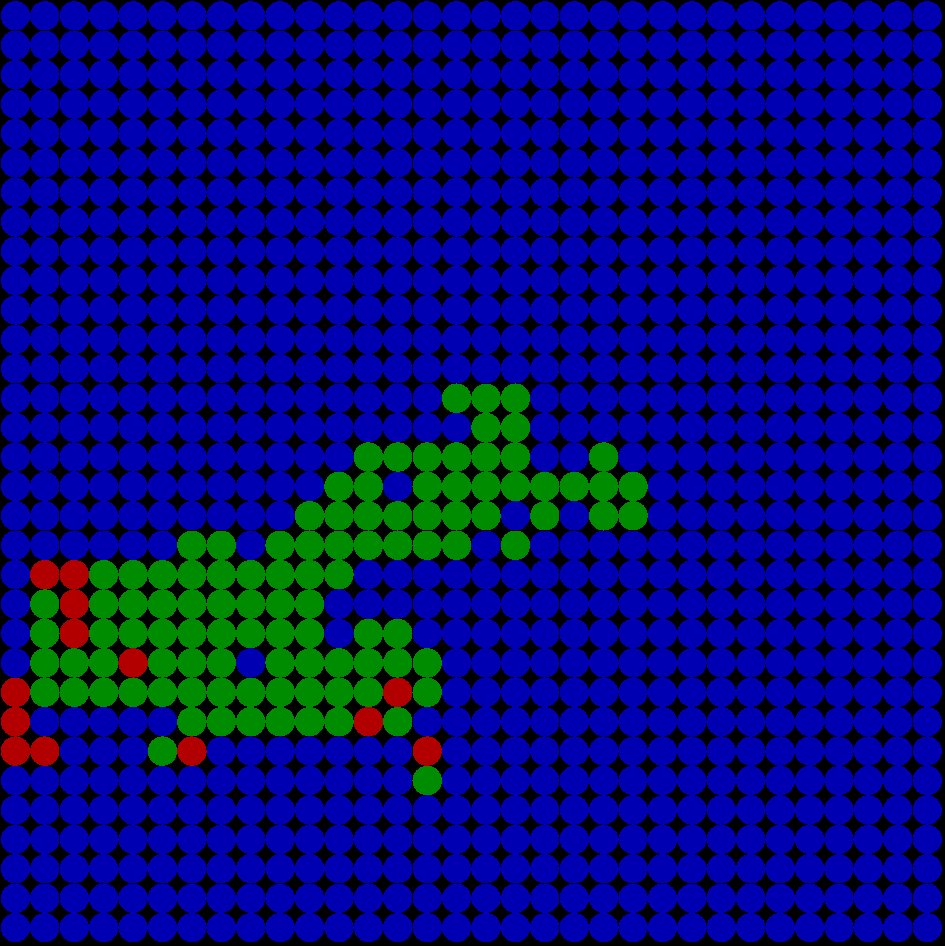
\includegraphics[width=.7\textwidth, angle=0]{./../shared/fig/randomness/SIR_32x32_200time_01delta_noSS.png}
			\caption{$\Delta t = 0.1$, no super-sampling}
			\label{fig:sir_abs_timeDeltas_randomness_dt01}
		\end{subfigure}
	
		& 
		
		\begin{subfigure}[b]{0.4\textwidth}
			\centering
			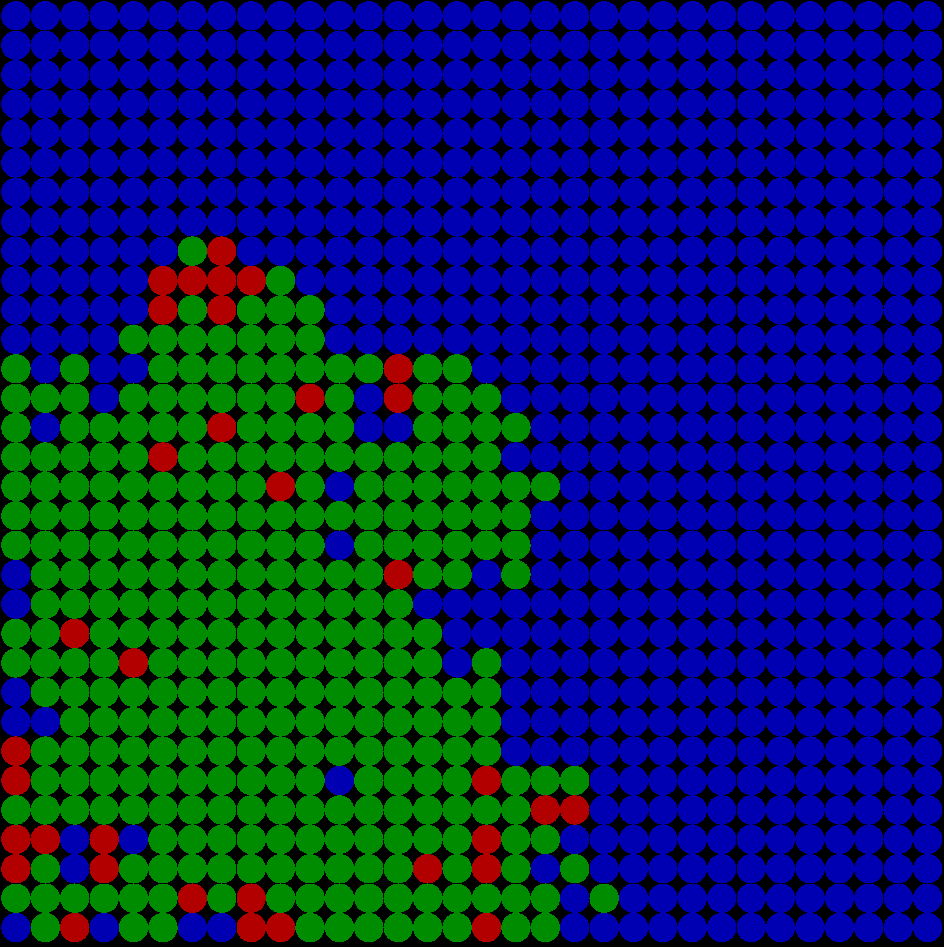
\includegraphics[width=.7\textwidth, angle=0]{./../shared/fig/randomness/SIR_32x32_200time_001delta_noSS.png}
			\caption{$\Delta t = 0.01$, no super-sampling}
			\label{fig:sir_abs_timeDeltas_randomness_dt001}
		\end{subfigure}
		
		\\

		\begin{subfigure}[b]{0.4\textwidth}
			\centering
			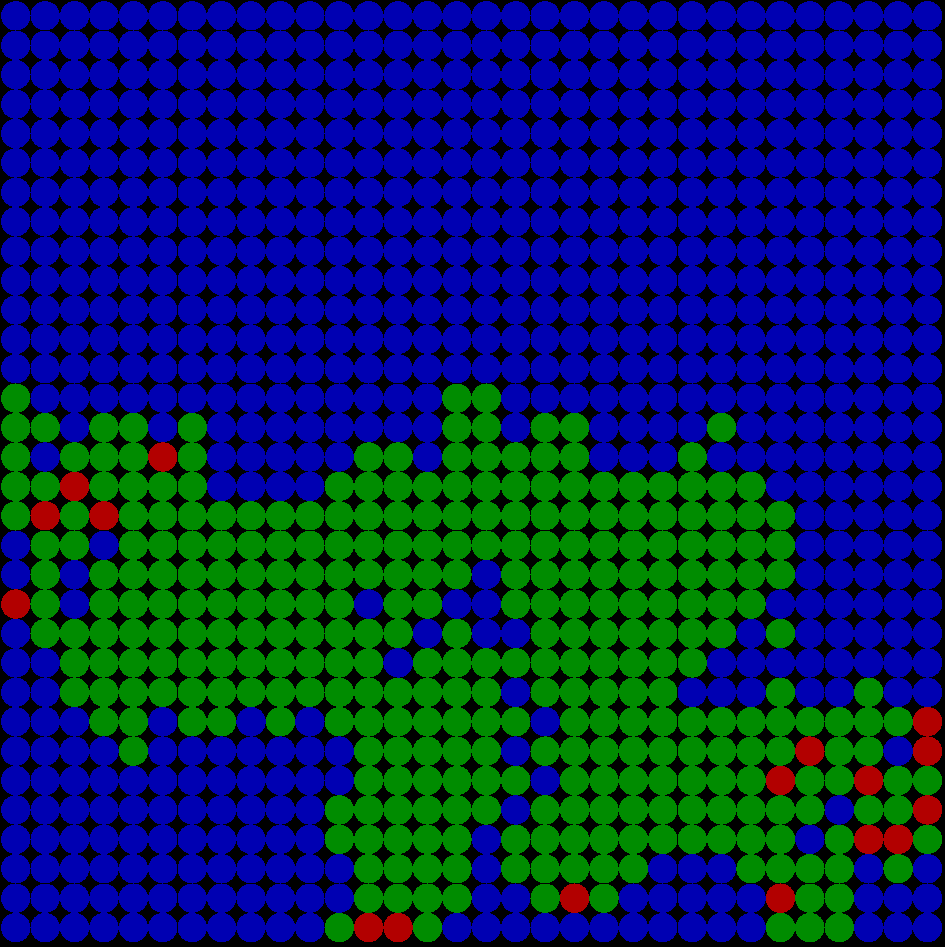
\includegraphics[width=.7\textwidth, angle=0]{./../shared/fig/randomness/SIR_32x32_200time_10delta_ss10.png}
			\caption{$\Delta t = 1.0$ with 10 super-samples}
			\label{fig:sir_abs_timeDeltas_randomness_dt10_ss10}
		\end{subfigure}
		
		&
		
		\begin{subfigure}[b]{0.4\textwidth}
			\centering
			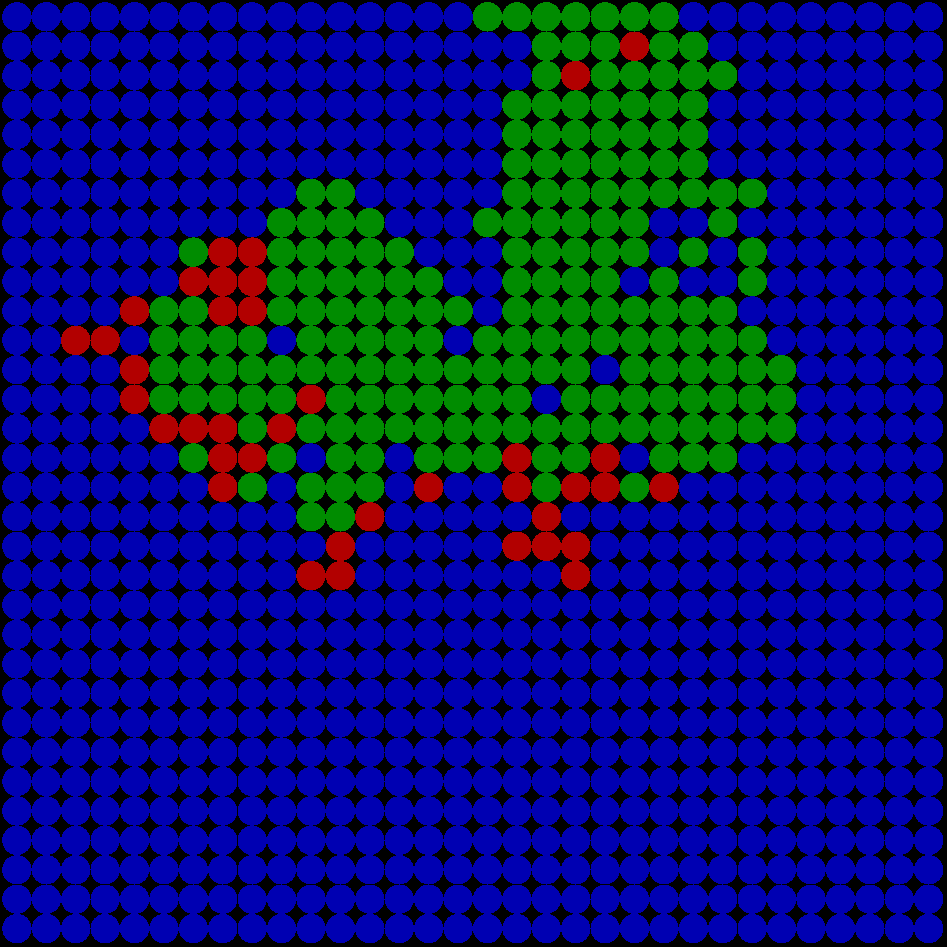
\includegraphics[width=.7\textwidth, angle=0]{./../shared/fig/randomness/SIR_32x32_200time_10delta_ss100.png}
			\caption{$\Delta t = 1.0$ with 100 super-samples}
			\label{fig:sir_abs_timeDeltas_randomness_dt10_ss100}
		\end{subfigure}
	\end{tabular}
	
	\caption{Comparing results on 32x32 grid after $t = 200$ but with different $\Delta t$ and different number of super-samples.}
	\label{fig:sir_abs_timeDeltas_randomness}
\end{center}
\end{figure*}